\def\year{2018}\relax
%File: written.tex
\documentclass[letterpaper]{article} %DO NOT CHANGE THIS
\usepackage{aaai18}  %Required
\usepackage{times}  %Required
\usepackage{helvet}  %Required
\usepackage{courier}  %Required
\usepackage{url}  %Required
\usepackage{graphicx}  %Required
\frenchspacing  %Required
\setlength{\pdfpagewidth}{8.5in}  %Required
\setlength{\pdfpageheight}{11in}  %Required

\usepackage[utf8]{inputenc}
\usepackage{multicol, blindtext}
\usepackage{url}
\graphicspath{{./Figures/}}

%PDF Info Is Required:
  \pdfinfo{
/Title (CS5751 Project Report)
/Author (UMD Student)}
\setcounter{secnumdepth}{0}  
 \begin{document}
% The file aaai.sty is the style file for AAAI Press 
% proceedings, working notes, and technical reports.
%
\title{Bitcoin Price Forecasting with Support Vector Machine \\and Autoregressive Integrated Moving Average Model}
\author{Benjamin Carpenter, Shuning Jin, Jacob Pauly, Tristan Larsin\\
University of Minnesota Duluth\\ %Department of Computer Science
1049 University Drive\\
Duluth, Minnesota 55812\\
}
\maketitle


% \begin{abstract}
% AAAI creates proceedings, working notes, and technical reports directly from electronic source furnished by the authors. To ensure that all papers in the publication have a uniform appearance, authors must adhere to the following instructions.
% \end{abstract}

% \noindent Congratulations on having a paper selected for inclusion in an AAAI Press proceedings or technical report! This document details the requirements necessary to get your accepted paper published using \LaTeX{}. If you are using Microsoft Word, instructions are provided in a different document. If you want to use some other formatting software, you must obtain permission from AAAI Press first.

%%%%%%%%%%%%% 1 Introduction %%%%%%%%%%%%%%%
\section{1 Introduction}

In this project, we will use machine learning methods to predict bitcoin prices based on historical market data. It would empower businesses and individuals to make better financial investments. It would also assist in understanding the probabilities of risk and reward for specific investments. We are specifically interested in investigating two methods: Autogressive Integrated Moving Average (ARIMA) and Support Vector Machine (SVM). The objectives of the project are as follows:
\begin{itemize}
\item Implementing ARIMA and SVM algorithms for time series forecasting
\item Using the algorithms to predict future prices based on previous prices
\item Evaluating and comparing the performance of the two algorithms
\end{itemize}
In the rest of the paper, we will introduce related work in Section 2, our proposed work in Section 3, experimental evaluation in Section 4, and conclusions and future work in Section 5.

%%%%%%%%%%% 2 Related Work %%%%%%%%%%%%%%%
\section{2 Related Work }

The work proposed by Zhang et al. \cite{zhang} is a hybrid methodology to combine the linear ARIMA and nonlinear ANN models for time series forecasting to improve performance. The empirical results with three real data sets suggest that the hybrid model outperforms its component model, and Canadian lynx data shows 19\% decrease in MSE and 8\% decrease in MAD.
\par
In a 2014 white paper \cite{leung}, a team from the University of Manitoba uses structural support vector machines (SSVMs) in an attempt to predict future stock market prices. SSVMs are a specialized form of supervised learning algorithm that can perform linear and non-linear regression to predict similar outcomes from past data \cite{tsochan}. In their results, they found the algorithm was performing with 78\% accuracy.
\par
In 2017, Facebook developed Prophet \cite{taylor}, which is a powerful tool for time series forecasting available in Python and R. Prophet is aimed at efficiently producing high quality forecasts with large number of time series data points. They used the generalized additive model (GAM), which is based on time series decomposition. Three main components are used: trend, seasonality, and holiday. GAM has great flexibility when used non-parametrically.
\par
Autoregressive Integrated Moving Average (ARIMA) was used by Vinay et al. \cite{vinay} to predict road-traffic volume. ARIMA is used for short-term and long-term historical data. There are several variations of ARIMA that are best suited for given problems. This research tested all of the variations to compare the different accuracies of his road-traffic volume predictions. Some variations have more overhead than others, but lack accuracy. Based purely on accuracy ARIMA-GARCH outperformed all other variations of ARIMA.
\par
In a 2016 paper \cite{ved}, a team used a support vector machine (SVM) and kernel functions to forecast the stock market. They separated the stock market changes into two classifications, rising and declining. When rising, the value at $x-1$ is less than that at $x$. When declining, the value at $x+1$ is less than that at $x$. The types of SVM kernels used were linear, polynomial, and radial basis. The most accurate SVM kernel performed with an 88.34\% accuracy.
\par
Additional methods used by David Sheehan \cite{sheehan} including the long short term memory (LSTM) model, which is a type of deep learning that can predict cryptocurrency prices. LSTM models are well suited for time series data because loops in neural nets allow for persistent data. In essence, they can remember how time series data has behaved in the past. Sheehan decided to use the same Bitcoin dataset that we have chosen. This dataset includes Bitcoin’s details at a one-minute interval from January 2012 through January 2018. This provided him with six years of data. Testing his algorithm from July 1st, 2017 through November 1st, 2017 he received a mean absolute error (MAE) of 0.0392.
\par
In our project, we will apply SVM and ARIMA for bitcoin price prediction. While SVM and ARIMA have been widely applied for stock price forecasting, we want to investigate their predictive power in the context of bitcoin. Also, we are interested in comparing the performance of these two algorithms.


%%%%%%%%%%%%% 3 Proposed Work %%%%%%%%%%%%%
\section{3 Proposed Work}
In this section, we will discuss the two proposed algorithms: ARIMA and SVM, as well as evaluation metrics of model performance.
%%% 1 ARIMA %%%
\subsection*{3.1 Autoregressive Integrated Moving Average Model (ARIMA)}
ARIMA model is a generalization of ARMA model, with the form:
$$\phi(B)(1-B)^dX_t=\delta+\theta(B)w_t  \qquad for ~ t = 1,2,… $$
where $\delta = \mu(1-\sum_{i=1}^{p}\phi_i)$, $w_t$ is white noise with independent and identical distributions, $\phi$ and $\theta$ are vectors of unknown fixed regression coefficients, and B is back-shifting operator defined as $B^dx_t=x_{t-d}$.

\subsubsection*{(i) Model Specification}~\\
The ARIMA$(p,d,q)$ model consists of three parts:
\par
Autoregression of order $p$: AR assumes current value $x_t$ is correlated with p past values, where p denotes the number of time lags. The autoregressive process models the trend of $x_t$.
\par
Moving average of order $q$: MA assumes current value $x_t$ is correlated with q recent white noises. The moving average smoother is to remove white noise in data and helps discover underlying long-term trend.
\par
Differencing of order $d$: time series are usually modeled by a stationary component and a nonstationary component. Performing differencing is to remove trend and produce stationarity. First difference is defined as $\nabla x_t=x_t-x_{t-1}$.

\subsubsection*{(ii) Model Fitting}~\\
Given $p,d,q$ order for ARIMA model, we shall firstly do d-order differencing and reduce it to ARMA(p,q). Secondly, we focus on estimating parameters $\phi$ and $\theta$ in ARMA model. There are two typical techniques for such estimation: Yule-Walker estimation and maximum likehood estimation.

%%% 2 SVM %%%
\subsection*{3.2 Support Vector Machine (SVM)}

SVM constructs a hyperplane or set of hyperplanes in a high-dimensional space, which can be used for classification, regression. It allows flexible mapping of high dimensional features to capture non-linear relationships with regularization to avoid over-fitting. Our goal is to draw a dividing line between classes which maximizes the the space between the line and the nearest points (known as the 'margin'). In sigma notation, we want to minimize $W(\alpha)$:
$$ W(\alpha) = \sum_{i=1}^l \alpha_i +
    \frac{1}{2} \sum_{i=1}^l \sum_{j=1}^l y_i y_j \alpha_i \alpha_j (x_i \cdot  x_j) $$

\noindent
where $\alpha$ is the vector of l non-negative Lagrange multipliers to be determined, and C is a constant. \\ \\ In order to construct $W$, Lagrange multiplication technique is applied to an optimization problems bounded by a constraint. Here, the constraint that must be satisfied is:
$$ \sum_{i=1}^l y_i \alpha_i = 0 \qquad 0 \le \alpha_i \le C \quad \forall i$$

\noindent
Note that only the closest points to the hyperplane (dividing line) are important for the problem. We could remove all other points and arrive at the same solution. Those points and their derived vectors are the 'support vectors' in SVM. By adding dimensions, we can apply SVM to many independent variables.


%%% 3 Evaluation Metrics %%%
\subsection*{3.3 Evaluation Metrics}

\subsubsection*{(i) Goodness of Fit}~\\

\textbf{Akaike’s Information Criterion (AIC)}
$$AIC = log\hat{\sigma}_k^2+\frac{n+2k}{n}$$

\textbf{AIC, Bias Corrected (AICc)}
$$AICc = log\hat{\sigma}_k^2+\frac{n+k}{n-k-2}$$

\textbf{Bayesian Information Criterion (BIC)}
$$BIC = log\hat{\sigma}_k^2+\frac{klog n}{n}$$

\textbf{Mean Square Error (MSE)}
$$MSE = \frac{SSE(k)}{n-k}$$
where $\hat{\sigma}_k^2$ is the maximum likelihood estimator of variance, SSE is residual sum of squares, k is the number of parameters, and n is the number of observations.

\subsubsection*{(ii) Prediction Accuracy}~\\

\textbf{Mean Absolute Percentage Error (MAPE)}
$$M = \frac{100}{n}\sum_{t=1}^{n}|\frac{A_t-F_t}{A_t}|$$
where $A_t$ is the actual value and $F_t$ is the forecast value.

%%%%%%%%%%%%%%%% 4 Experimental Evaluation %%%%%%%%%%
\section{4 Experimental Evaluation}
\subsection{4.1 Dataset}
We use a dataset of historical exchanges of Bitcoin from January 1, 2012 to January 8, 2018 (\citeauthor{bitcoin_set}). The data is based on every minute update, and contains 3,161,057 observations in total. It has 8 attributes: timestamp (in Unix time), open, high, low, close, volume in BTC, volume currency, and weighted price. The csv file has a size of 212.8 MB.

%\subsection{4.2 Experiment Parameter}

\subsection{4.2 Preprocessing}
The original dataset is based on every minute data from 2012-01-01 to 2018-01-08. Initially, we transform it to daily data by adopting the observations on 00:00 for each day. We use the close price as both the response variable and the explanatory variable. Figure \ref{figure:2012-2018} shows the trend in early years is relatively trivial. Thus, we decide to only use data from 2017-01-01 to 2018-01-01, which has 366 observations. To stabilize the variance, log transform is applied. The data after preprocessing is shown in Figure \ref{figure:2017-2018 log}.



%Since 1 data point is lost due to previous differencing, we have 365 data in total, with the first 328 for train and the last 37 for test. 
%Second, we fit the model with training data. The train error is measured by MSE = 0.002159. Third, we make m-step-ahead long range forecast based on historical (train) data, with m = test size = 37. By comparing predicted values with test data, we derive test error in two ways. The test MSE is 0.006412. And MAPE is 23.40647.
%Then, we fit the model with training data. The train error is measured by MSE. 

\subsection{4.3 Evaluation Method}
To evaluate the models performance, we divide the data into training set and testing set using a 90:10 split. Due to the nature of time series data, we could not do random sampling here. We make forecasts based on historical data, and test error is measured by MSE and MAPE. There are two types of forecast: one-step-ahead and m-step-ahead (long range). In one-step-ahead forecast, each next point is predicted based on past p (autoregressive order) true values. In m-step-ahead forecast, only the first 90\% points are used for fitting, and the future points are predicted by recursive one-step-ahead forecast. In conjunction with past true values, newly predicted values are also used to prophesy the next immediate point, and the procedure repeats m times.

\subsection{4.4 ARIMA Experiment}
\subsubsection*{4.4.1 Model Building}~\\
There are three hyperparameters in ARIMA$(p,d,q)$model. \\
We want to identify the differencing order d, and sample ACF $\hat\rho(h)$ serves a criterion - that is, slow decay in ACF indicates a need for differencing. Since the ACF of our data (Figure \ref{figure:acf1}) shows such pattern, we do first differencing. After that, the ACF (Figure \ref{figure:acf2}) suffices and no futher differencing is needed. Hence, we decide d=1. The log first difference $\nabla log(x_t)$ is also called return or growth rate,  shown in Figure \ref{figure:return}.


%%%%%%%%%%%
%% plot for 2012-2018, 2017-2018 log tranform

\begin{figure}
    \includegraphics[width=\linewidth]{2012-2018.png}
    \caption{2012-2018 Bitcoin Daily Close Price}
    \label{figure:2012-2018}
\end{figure}

\begin{figure}
    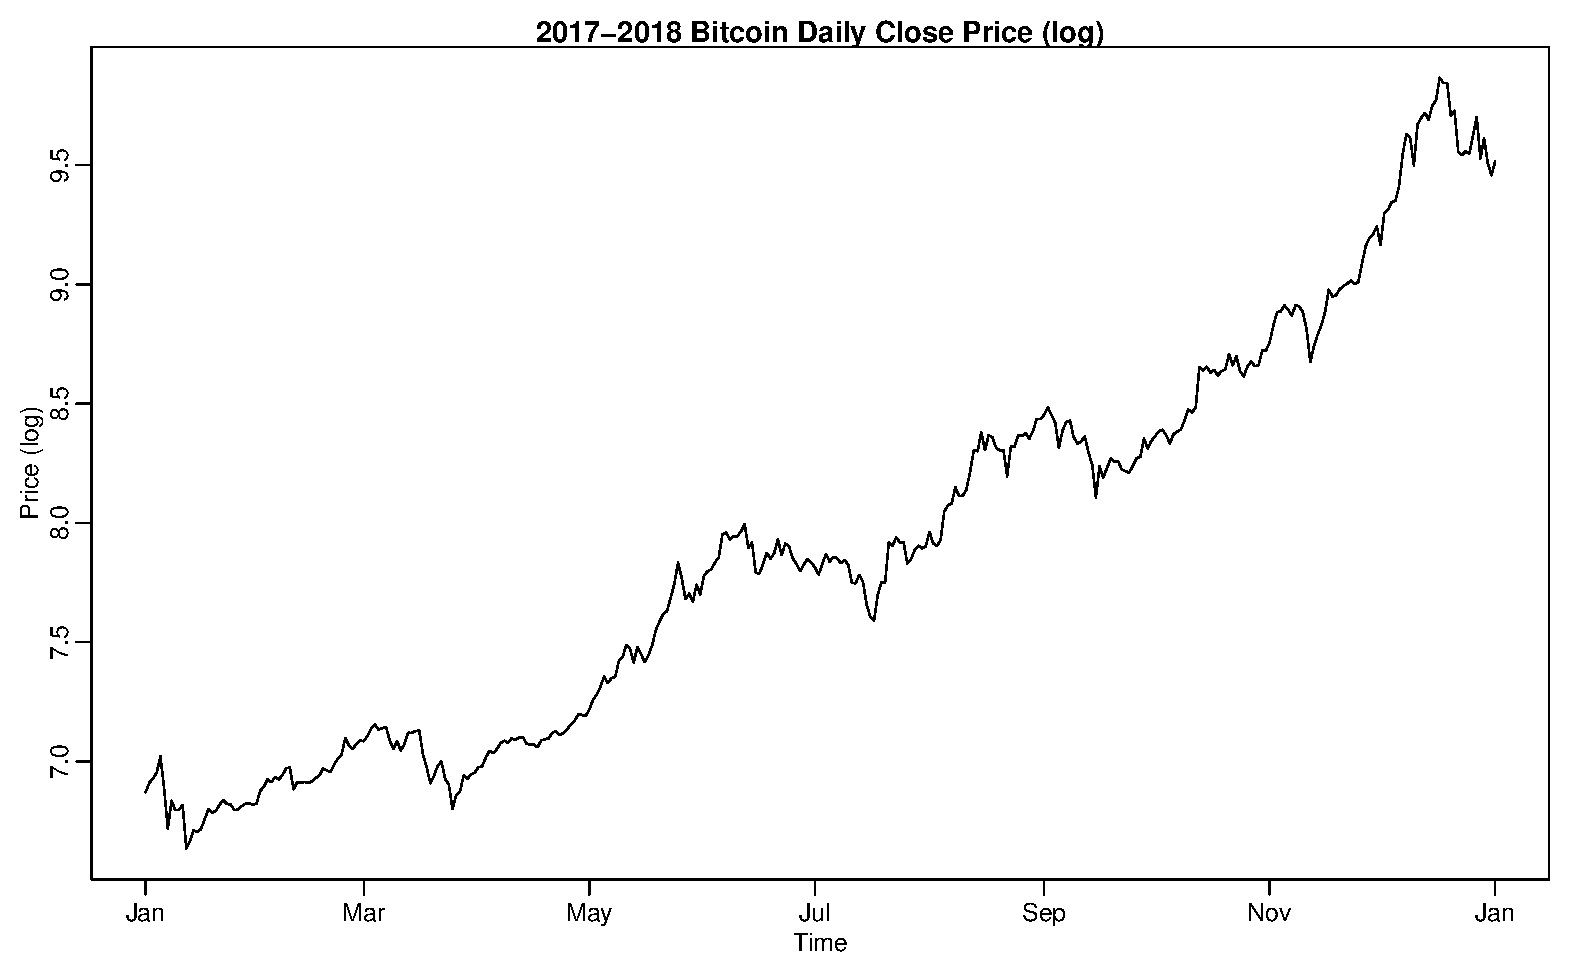
\includegraphics[width=\linewidth]{2017-2018_log.eps}
    \caption{2017-2018 Bitcoin Daily Close Price with Log Transformation}
    \label{figure:2017-2018 log}
\end{figure}
%%%%%%%%%%%%
%% ACF1, first differenced data

\begin{figure}
    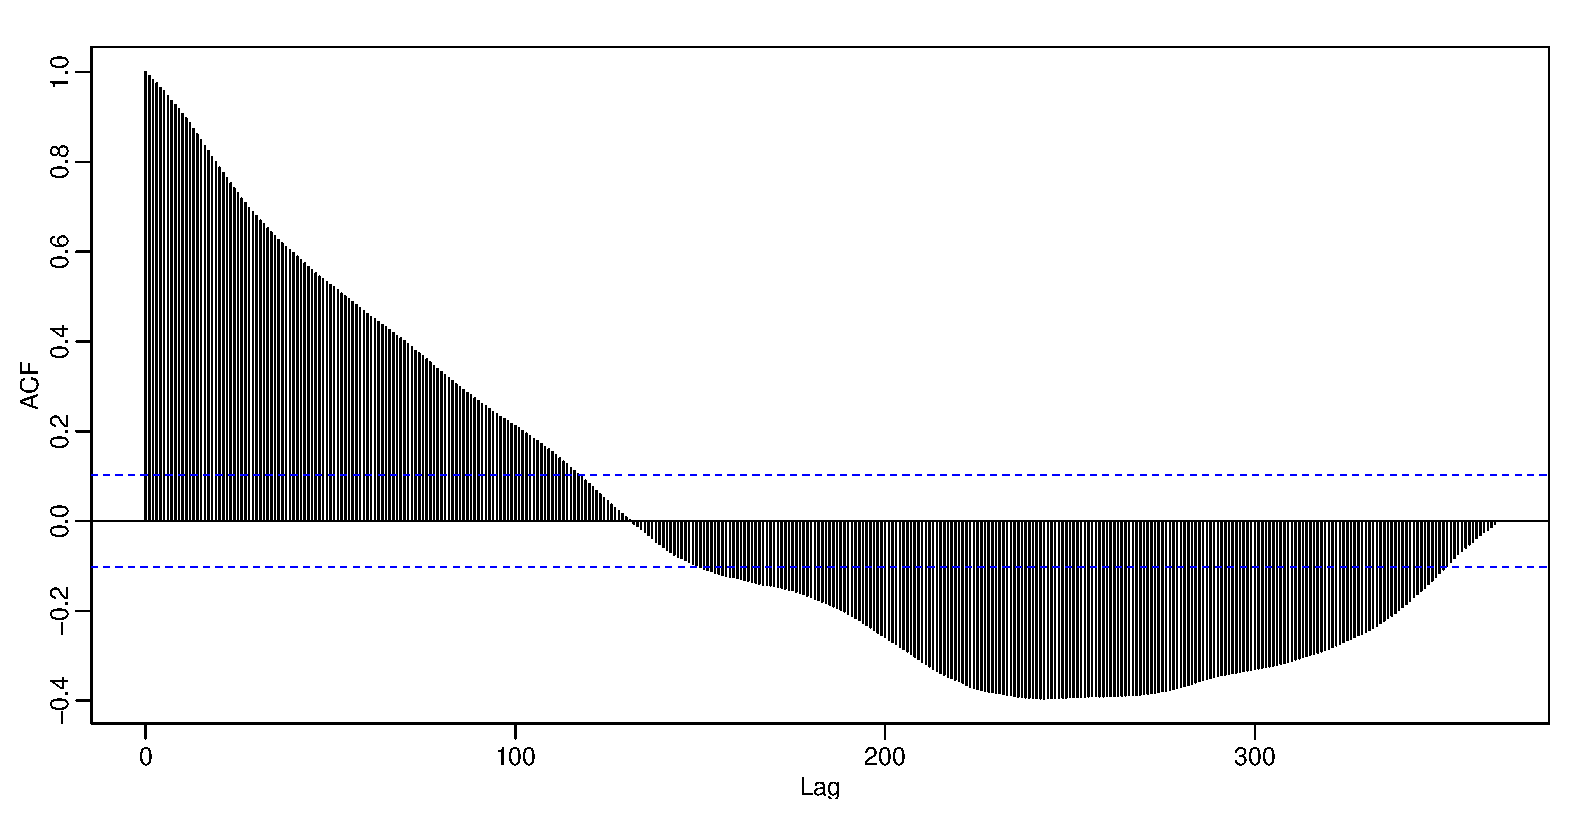
\includegraphics[width=\linewidth]{acf1.eps}
    \caption{ACF - Without Differencing}
    \label{figure:acf1}
\end{figure}

\begin{figure}
    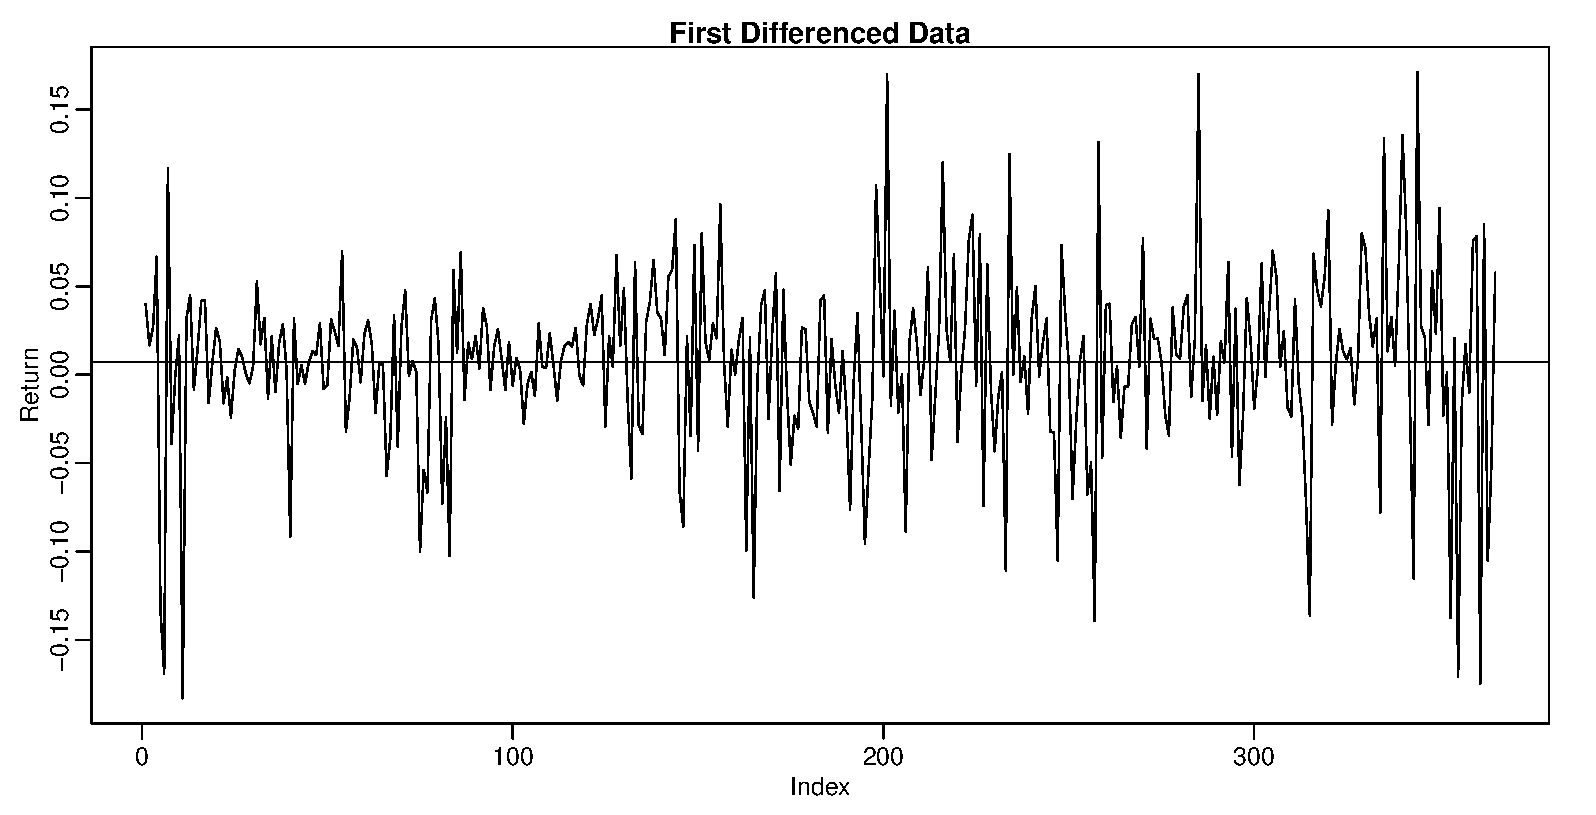
\includegraphics[width=\linewidth]{return.eps}
    \caption{Log First Differenced Price}
    \label{figure:return}
\end{figure}
%%%%%%%%%%%
%%  ACF2, PACF2

\begin{figure}
    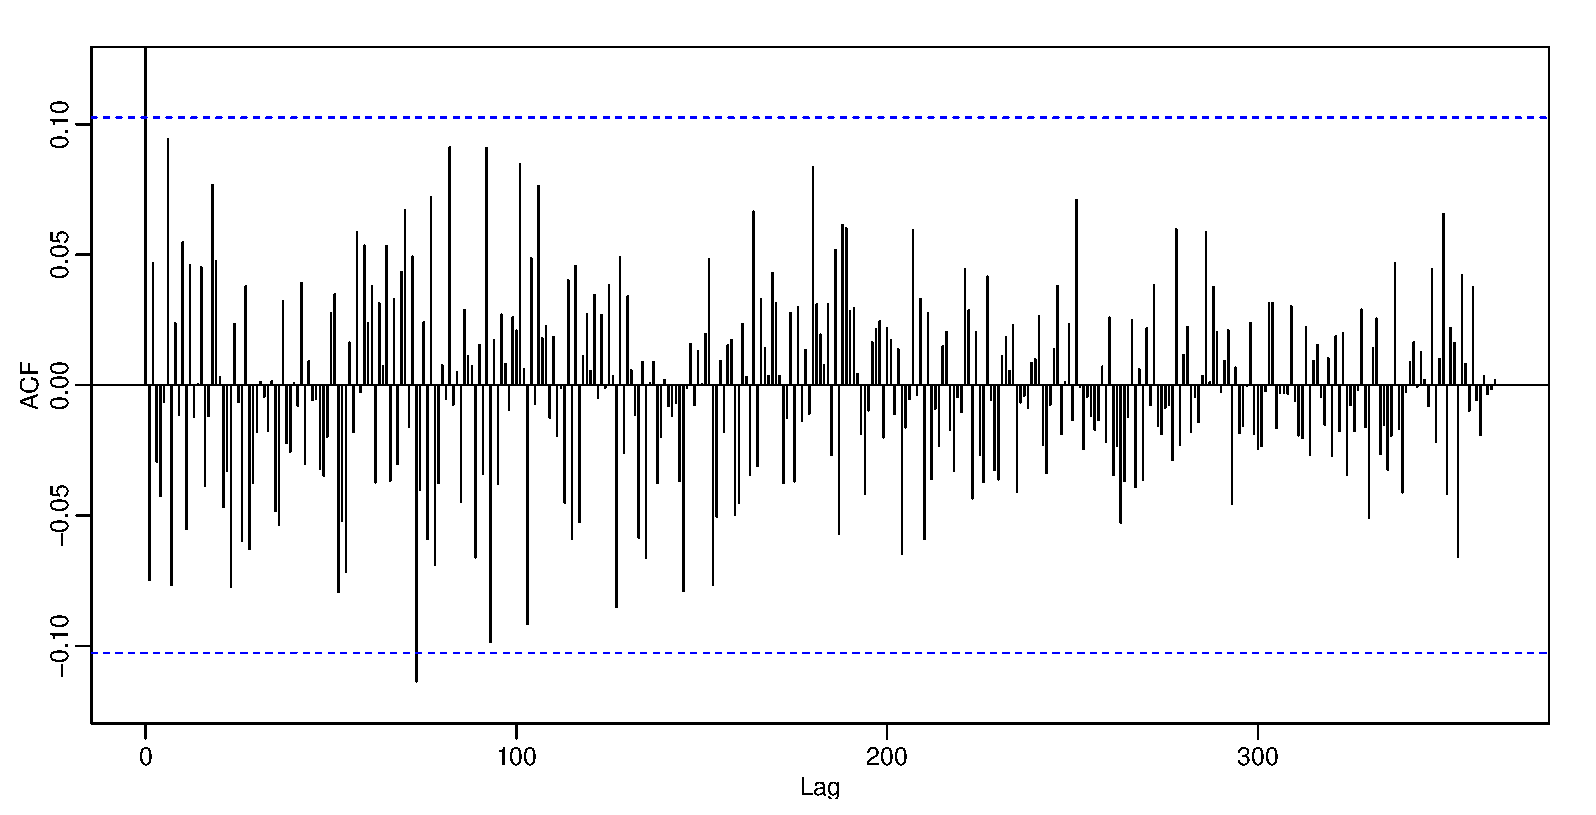
\includegraphics[width=\linewidth]{acf2.eps}
    \caption{ACF - First Differencing}
    \label{figure:acf2}
\end{figure}

\begin{figure}
    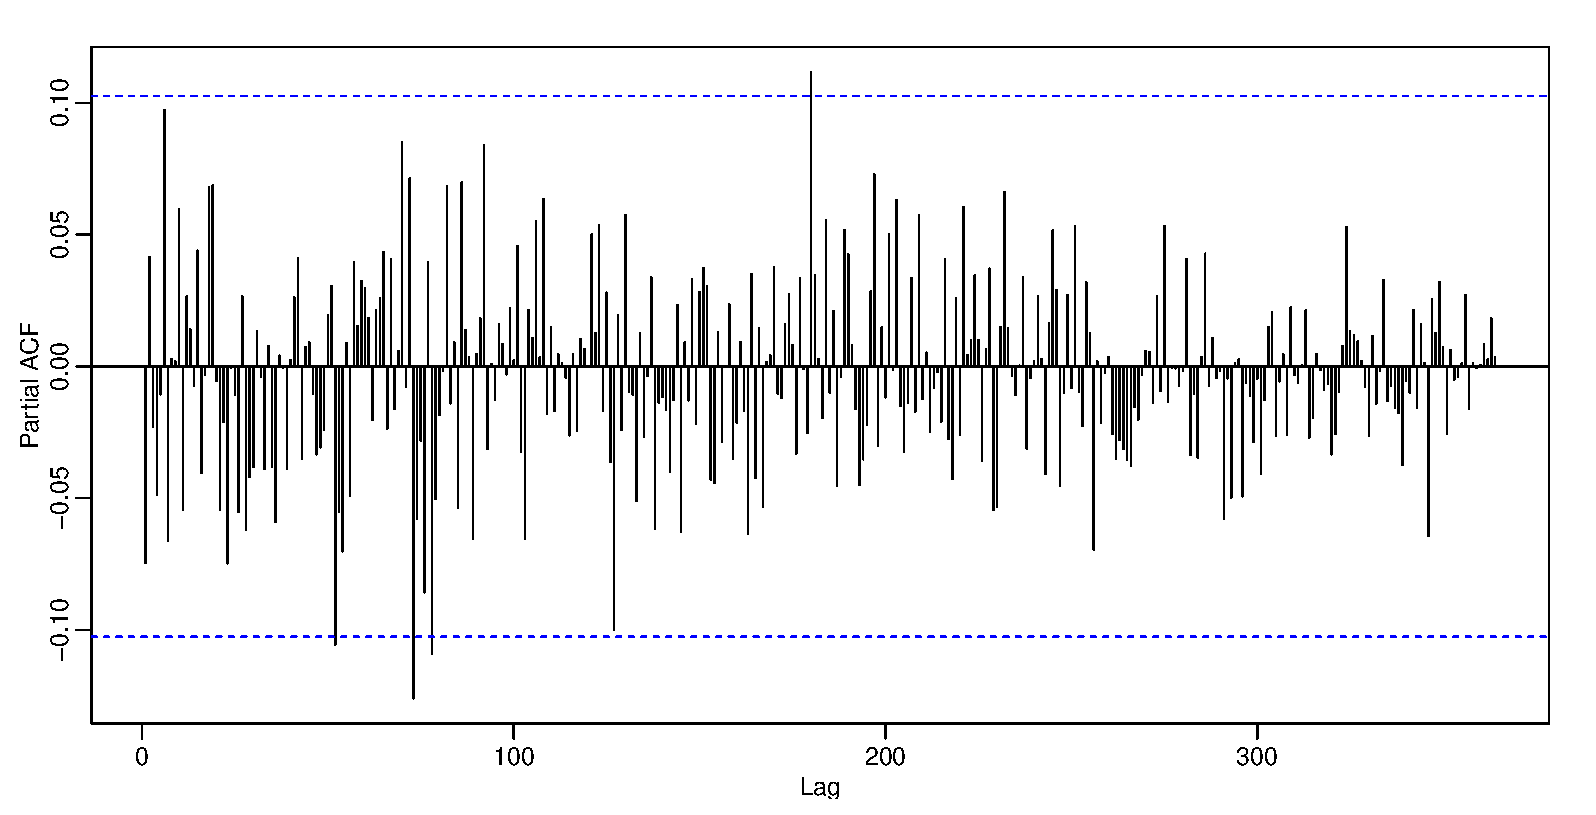
\includegraphics[width=\linewidth]{pacf2.eps}
    \caption{PACF - First Differencing}
    \label{figure:pacf2}
\end{figure}
%%%%%%%%%%%

We also need to identify the autoregressive order p and moving average order q. Above all, we need to determine if p=0 or q=0, which correspond to MA(q) or AR(p) respectively. We use the sample ACF and PACF behavior as a guide. Since there are no cut off after certain lags, and both ACF (Figure \ref{figure:acf2}) and PACF (Figure \ref{figure:pacf2}) tail off, we can conclude p and q are nonzero, leading to ARMA(p,q) model. For simplicity, we assign p=1 and q=1. That is, we adopt ARMA(p=1,q=1) for the first differenced data, which corresponds to ARIMA(p=1,d=1,q=1) for the original log transformed data. The model adequency will be more rigorously examined below.


\subsubsection*{4.4.2 Model Checking}~\\
With all three hyperparameters specified, we carry out preliminary model checking by residual analysis. Applying the data, the 'sarima' method in 'astsa' package gives 4 diagnostic plots (Figure \ref{figure:diagnosis}) of standardized residuals

$$ e_t = \frac{x_t - \hat{x}_{t}^{t-1}} {\sqrt{\hat{P}_{t}^{t-1}}} $$
where $\hat{x}_{t}^{t-1}$ is the one-step-ahead prediction of $x_t$,
and $\hat{P}_{t}^{t-1}$ is the estimated one-step-ahead error variance. \\

\par
(a) Ideally, the residuals should have iid distribution with $\mu=0$ and $\sigma^2=1$. The time plot shows no obvious patterns and the mean is around 0. But a few values exceed 3 standard deviations in magnitude, which could be outliers.
\par
(b) To check the assumption of randomness, we inspect the sample ACF. There are no significantly large values, indicating no apparent departure from this assumption.
\par
(c) The normal Q-Q plot is heavy tailed. This means the assumption of normality may not strictly hold.
\par
(d) The p values for Ljung-Box Q-statistic are large (greater than 0.2), thus we do not reject the null hypothesis of model adequency.
\\ \\ Thus, we conclude that this model is suitable for our dataset in general.

%% residual analysis

%\begin{figure*}[ht]
%\centering
\begin{figure}
    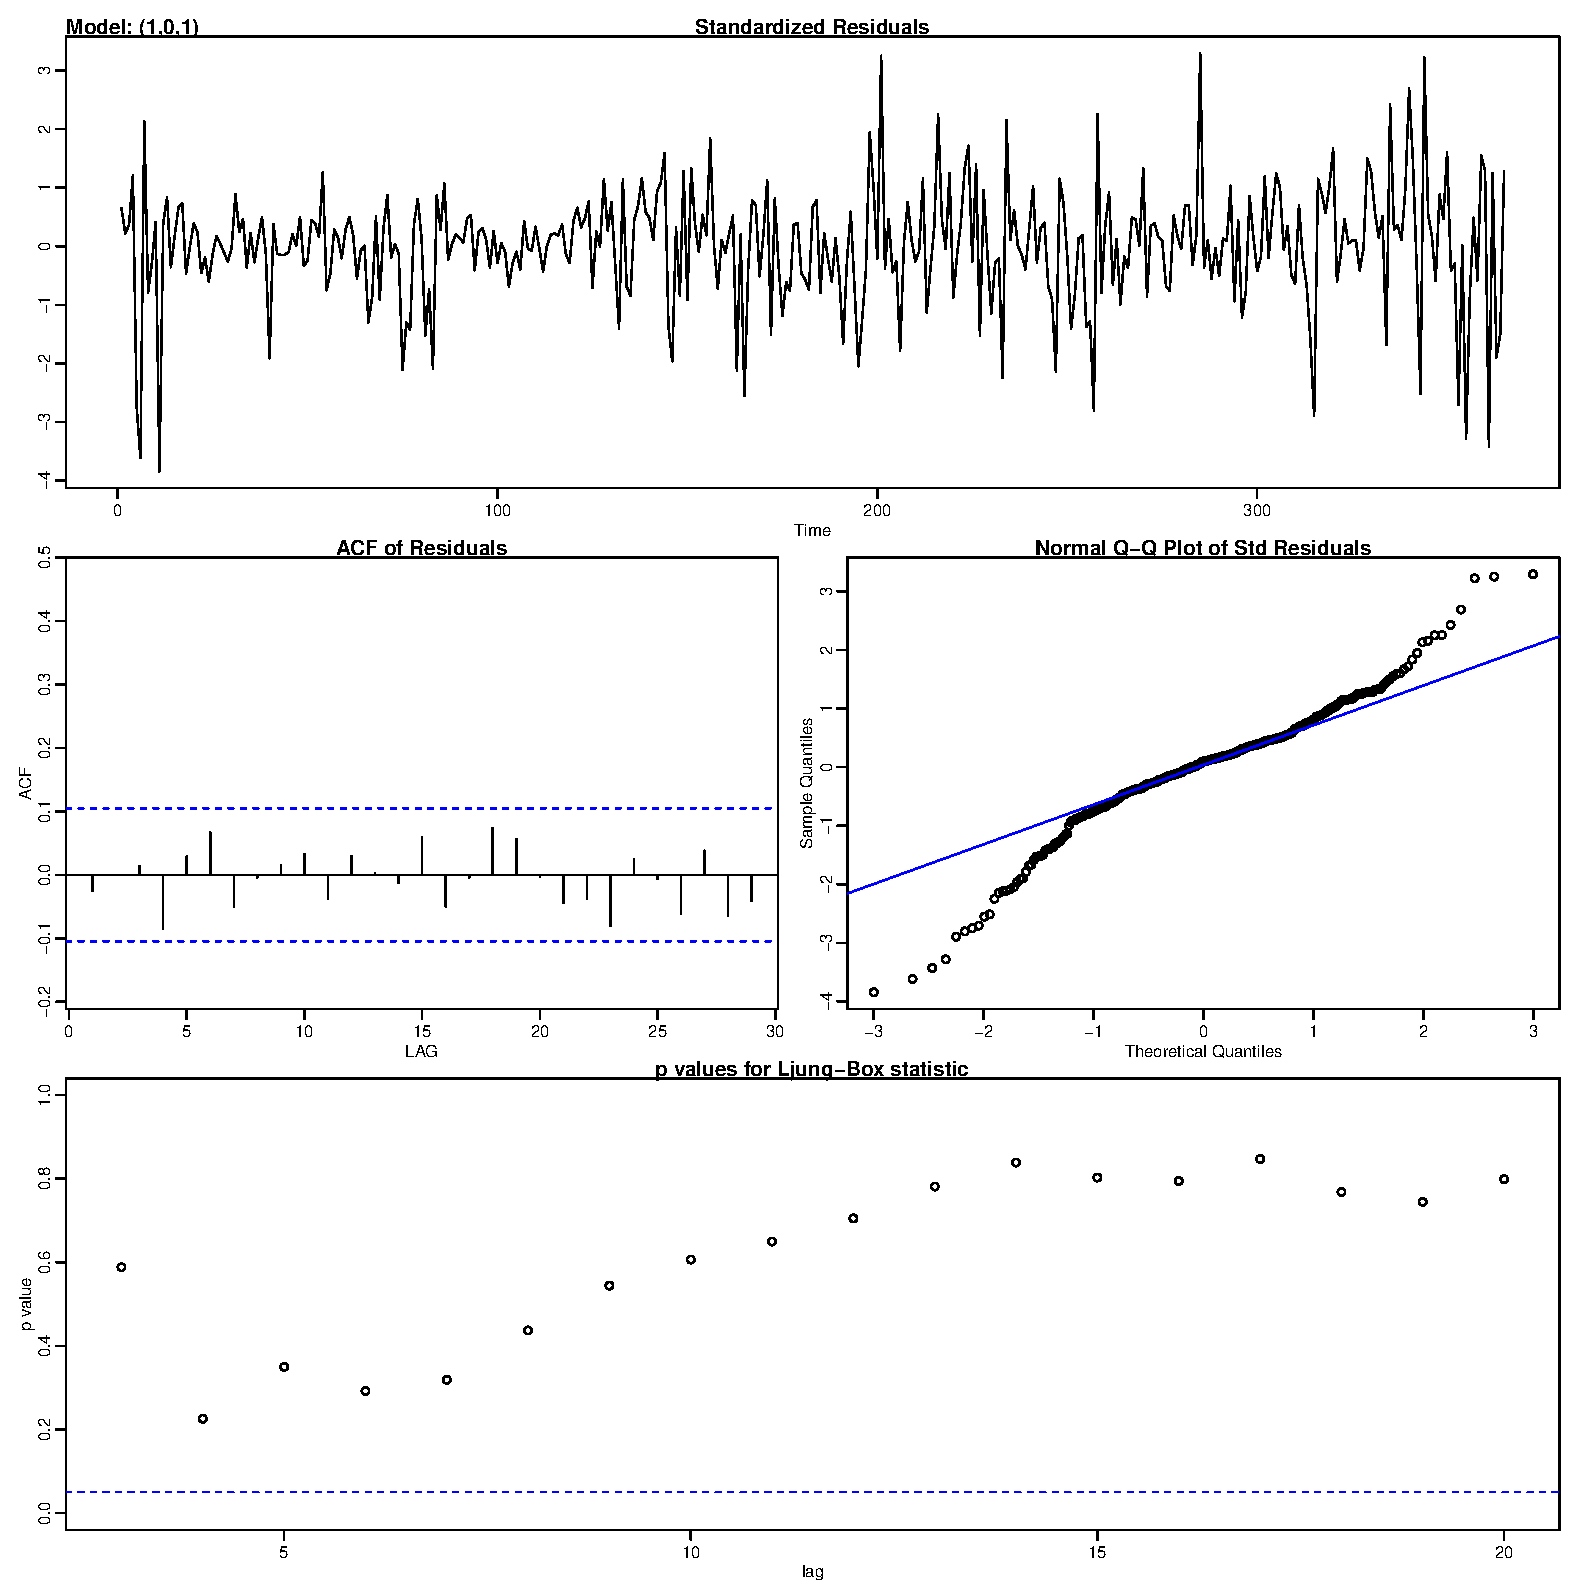
\includegraphics[width=\linewidth]{diagnosis.eps}
    \caption{Residual Diagnostics}
    \label{figure:diagnosis}
\end{figure}
%\end{figure*}

\subsubsection*{4.4.3 Model Performance}~\\
Since 1 data point is lost due to previous differencing, we have 365 data in total. First, after train-test split, we use first 328 for train and the last 37 for test. Second, we fit the model with training data. The train MSE is 0.0022. Third, one-step-ahead forecast gives MSE of 0.0063 and MAPE of 43.7934. In m-step-ahead  forecast with m = test size = 37, MSE is 0.0064 and MAPE is 23.4065. The forecast results for log first differenced price are shown in Figure \ref{figure:arima}.

\begin{figure}
    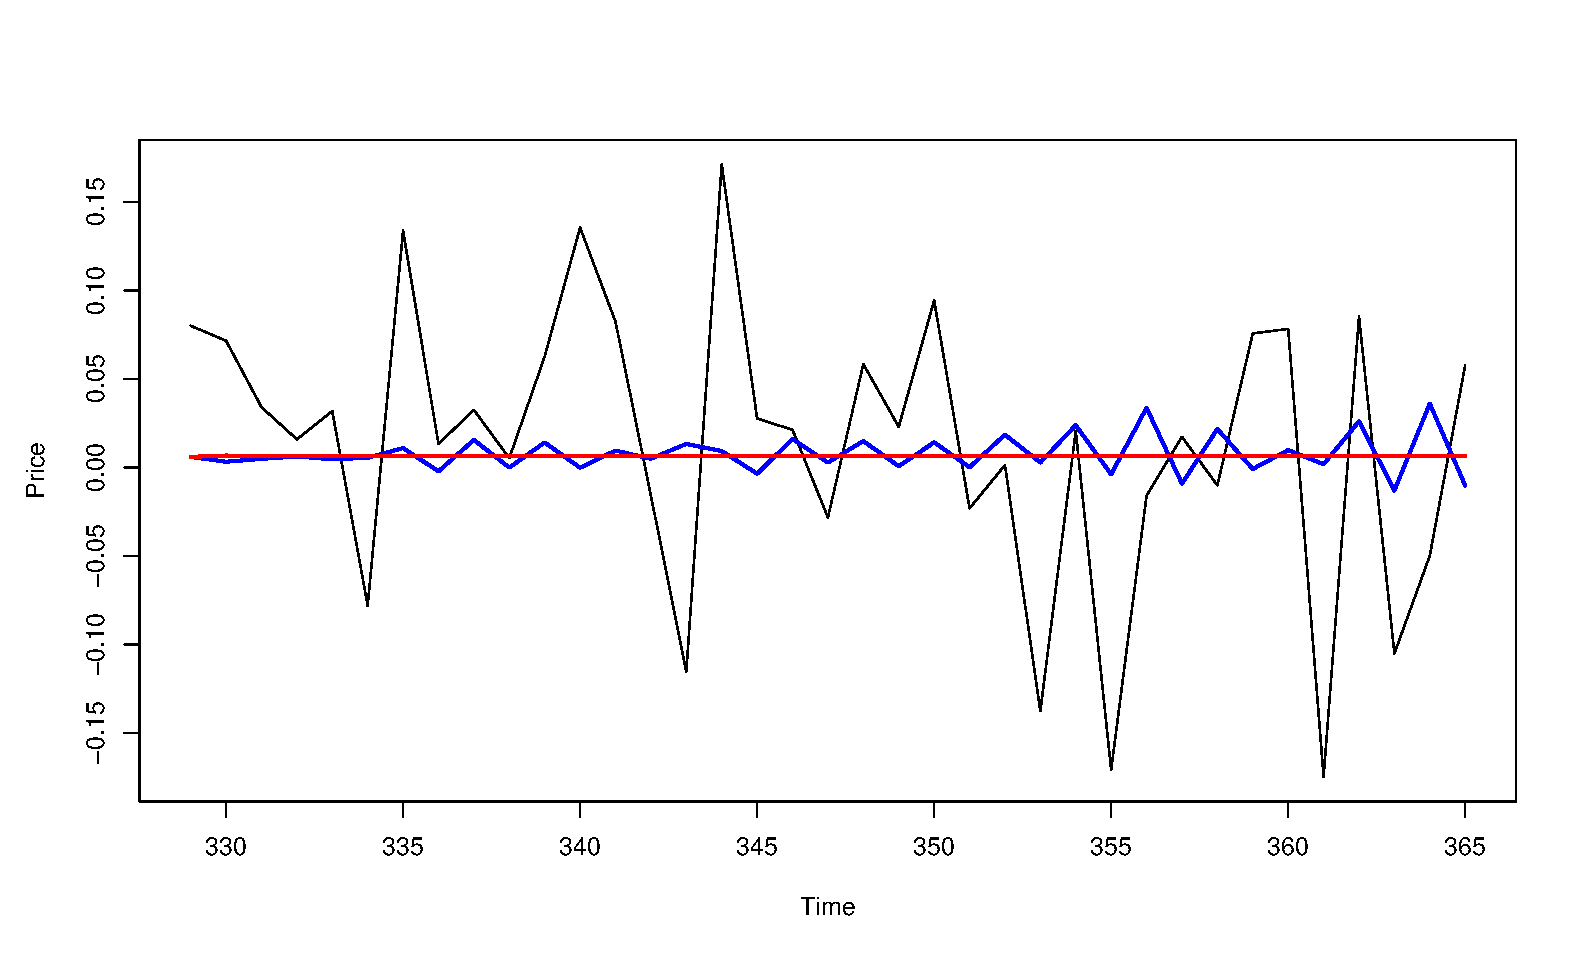
\includegraphics[width=\linewidth]{arima_fore.eps}
    \small\centering
	Black: true; Blue: one-step-ahead; Red: m-step-ahead.
    \caption{ARIMA Forecast for Log First Differenced Price}
    \label{figure:arima}
\end{figure}

\begin{figure}
    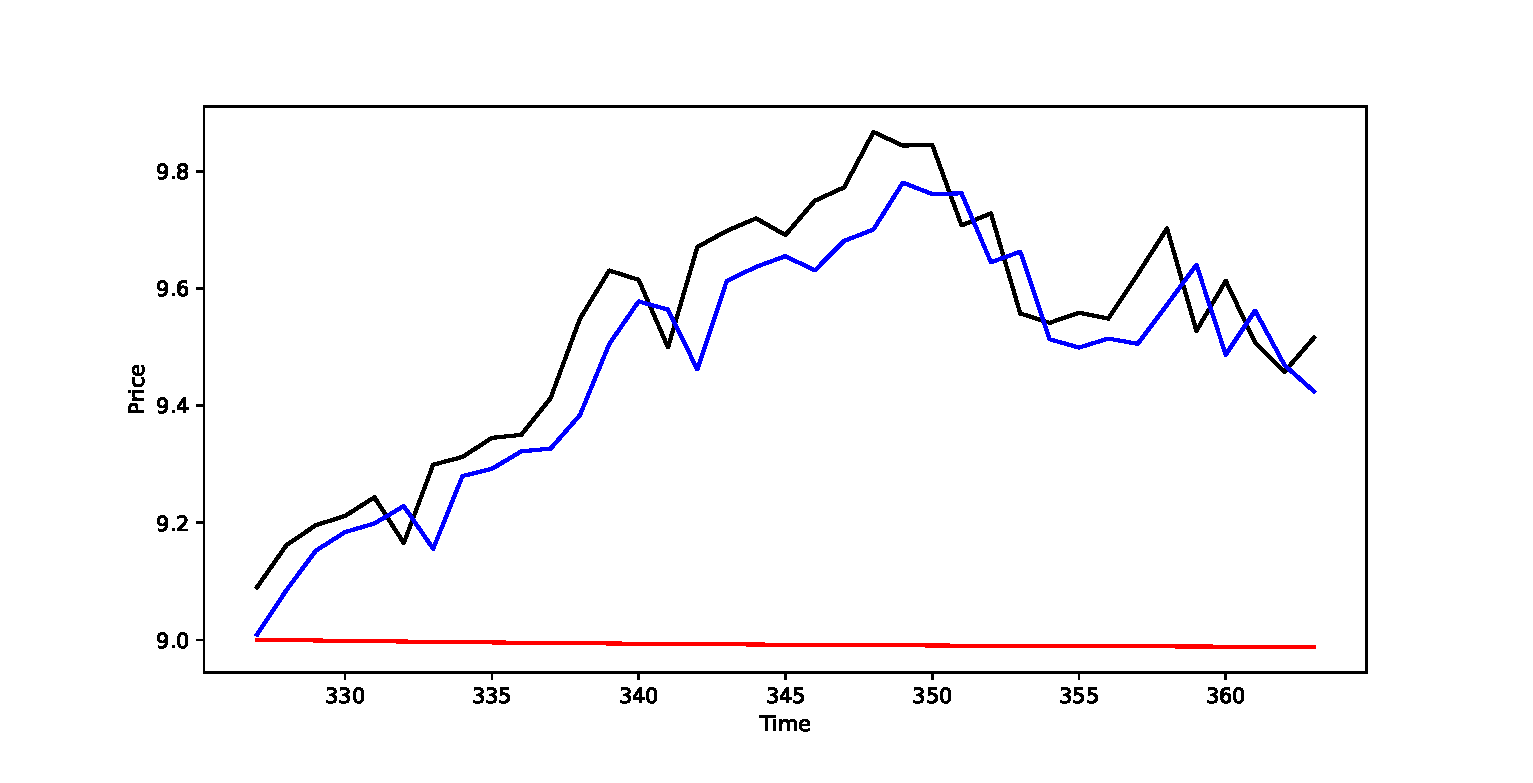
\includegraphics[width=\linewidth]{svm_fore.eps}
    \small\centering
    Black: true; Blue: one-step-ahead; Red: m-step-ahead.
    \caption{SVM Forecast for Log Price}
    \label{figure:svm}
\end{figure}

\subsection{4.5 SVM Experiment}
\subsubsection*{4.5.1 Model Building}~\\
When applying SVM to time series data, we need to integrate autoregression of order $p$. We choose p=1 to comply with ARIMA experiment. In this experiment, we adopt SVM with Radial Basis Function (RBF) kernel, using parameters $C$=100, $\gamma$=0.02, and $\epsilon$=0.01.


\subsubsection*{4.5.2 Model Performance}~\\
Since 1 data point is lost in autoregression of order 1, we have 365 data in total. First, after train-test split, we use first 328 for train and the last 37 for test. Second, we fit the model with training data. The train error is measured by MSE = 0.0022. Third, one-step-ahead forecast gives MSE of 0.0086 and MAPE of 0.8527. In m-step-ahead  forecast with m = test size = 37, MSE is 0.3308 and MAPE is 5.5688. The forecast results for log price are shown in Figure \ref{figure:svm}.

The table \ref{table:1} is an example of referenced \LaTeX elements.
 
\begin{table}[h!]
\centering
\begin{tabular}{||c c c c||} 
 \hline
 Col1 & Col2 & Col2 & Col3 \\ [0.5ex] 
 \hline\hline
 1 & 6 & 87837 & 787 \\ 
 2 & 7 & 78 & 5415 \\
 3 & 545 & 778 & 7507 \\
 4 & 545 & 18744 & 7560 \\
 5 & 88 & 788 & 6344 \\ [1ex] 
 \hline
\end{tabular}
\caption{Table to test captions and labels}
\label{table:1}
\end{table}

TablesEx7.png


%%%%%%%%%%%% 5 Conclusions and Future Work %%%%%%%%%%%%%%
\section{5 Conclusions and Future Work}
For both ARIMA and SVM, the training errors are small. However, test errors are relatively large. One-step-ahead forecast is generally more accurate than m-step-ahead forecast. In fact, m-step-ahead prediction produces a sequence with very small changes, which is ineffective. In the future, we would like to try different strategies for long range forecast other than recursive one-step-ahead approach. Second, to make a reasonable comparison between ARIMA and SVM, it is necessary to transform the results to a consistent  differencing order in post-processing. Third, we want to explore other hyper-parameters to find optimal settings for the models, which may lead to higher prediction accuracy.

%%%%%%%%%%%%%%%%%%%%%%%%%%%%%%%%%%%%%%%
\bibliography{bibfile}
\bibliographystyle{aaai}

%\cite{shumway}


\end{document}
